\documentclass[11pt]{article}
\usepackage[margin=1in]{geometry}
\usepackage{amsmath,amssymb}
\usepackage{booktabs,graphicx}
\usepackage[T1]{fontenc}
\pagestyle{empty}
\setlength{\parindent}{0pt}
\setlength{\parskip}{6pt}

\begin{document}

\begin{center}
{\Large Homework 2}\\[4pt]
Zhengxin Lu
\end{center}

\section*{Problem 1}

\textbf{1(a)}
Write $g(x)=(g_1(x),g_2(x))\in\mathbb{R}^2$. Set
\[
f_\mu(x)=g_1(x),\qquad f_\sigma(x)=\log\big(1+e^{g_2(x)}\big)+\varepsilon,\quad \varepsilon=10^{-3}.
\]
The identity link leaves the mean unrestricted; softplus makes the standard deviation strictly positive.

\textbf{1(b)}
Under $Y_i\mid X_i=x_i\sim N(\mu_i,\sigma_i^2)$ with $(\mu_i,\sigma_i)=(f_\mu(x_i),f_\sigma(x_i))$, the negative log-likelihood is
\[
L(\theta)=-\frac1n\sum_{i=1}^n\log p_\theta(y_i\mid x_i)
=\frac1n\sum_{i=1}^n\left[\frac12\log(2\pi)+\log\sigma_i+\frac{(y_i-\mu_i)^2}{2\sigma_i^2}\right].
\]
The constant $\frac12\log(2\pi)$ can be dropped during training. The squared-residual term rewards fit, while $\log\sigma_i$ prevents the model from inflating its uncertainty.

\textbf{1(c)}
The data contain 523,554 trips with 7 standardized features and duration in minutes as the target. I use a random 70/15/15 split: 366,487 training, 78,533 validation and 78,534 test trips. The model is a PyTorch MLP $7\to128\to128\to128\to2$ with ReLU hidden layers and the links from 1(a), trained on the loss from 1(b) with Adam (learning rate $2\times10^{-3}$, batch size 2048) and early stopping on validation NLL.

Baselines: (i) a constant Gaussian with the training mean and standard deviation; (ii) linear regression; (iii) histogram gradient boosting; (iv) the same MLP trained with MSE. For (ii)--(iv), $\sigma$ is a constant equal to the standard deviation of the validation residuals. Test results:

\begin{center}
\begin{tabular}{lccccc}
\toprule
Model & RMSE & NLL & Accuracy & Brier & Log-loss\\
\midrule
Constant Gaussian & 7.69 & 3.459 & 99.57\% & 0.0043 & 0.0532\\
Linear regression, constant $\sigma$ & 7.47 & 3.430 & 99.57\% & 0.0043 & 0.0452\\
Gradient boosting, constant $\sigma$ & 3.88 & 2.774 & 99.68\% & 0.0029 & 0.0238\\
MLP (MSE), constant $\sigma$ & 3.68 & 2.721 & 99.69\% & 0.0029 & 0.0249\\
Heteroscedastic MLP & 3.93 & 2.622 & 99.62\% & 0.0032 & 0.0172\\
\bottomrule
\end{tabular}
\end{center}

The heteroscedastic MLP has the best Gaussian NLL and log-loss, but not the best RMSE or Brier score. This is expected: learning an input-dependent variance improves the fit of the predictive distribution, not necessarily the squared error of the mean. The predicted $\sigma$ has 5th/50th/95th percentiles of about 1.9/3.4/6.5 minutes.

\textbf{1(d)}
Under the fitted model,
\[
\hat p(x)=P(Y<45\mid X=x)=\Phi\!\left(\frac{45-f_\mu(x)}{f_\sigma(x)}\right),
\]
where $\Phi$ is the standard normal CDF. Thresholding at $0.5$ predicts ``under 45'' exactly when $f_\mu(x)<45$; the probability itself also depends on $f_\sigma(x)$.

\textbf{1(e)}
For each test trip let $z_i=1\{y_i<45\}$ and $p_i=\hat p(x_i)$. I report
\begin{gather*}
\text{Brier}=\frac1n\sum_i(p_i-z_i)^2,\qquad
\text{Acc}=\frac1n\sum_i1\{1(p_i\ge0.5)=z_i\},\\
\text{Log-loss}=-\frac1n\sum_i\big[z_i\log p_i+(1-z_i)\log(1-p_i)\big].
\end{gather*}
The heteroscedastic MLP gives Brier score 0.0032, log-loss 0.0172 and accuracy 99.62\%. Since 99.57\% of test trips are under 45 minutes, always predicting ``under 45'' already gives 99.57\% accuracy, so accuracy alone is not informative here. The model overstates very high probabilities: among the 75,602 trips with $p_i\in[0.999,1]$, the mean prediction is 0.99999 while the observed rate is 0.9992. This suggests that trip durations have a heavier right tail than the Gaussian allows.

\section*{Problem 2}

Quantity is heavy-tailed (median 6, 99th percentile 120, maximum 80,995), so all models predict $Z=\log(1+Y)$ with squared-error loss, and I report MSE on $Z$. This reduces the influence of a few very large orders.

\textbf{2(a)}
The 397,924 transactions contain 3,665 distinct StockCodes and 4,339 distinct CustomerIDs. One-hot encoding both features gives 8,004 columns with two nonzero entries per row. This is feasible as a sparse matrix, but a dense float32 matrix for the 278,546 training rows would take about 8.9 GB, and one-hot encoding gives the many rare levels noisy coefficients. This suggests lower-dimensional encodings such as target encoding or learned embeddings. I use a random 70/15/15 split: 278,546 / 59,689 / 59,689 rows. Predicting the training mean gives test MSE 1.014.

\textbf{2(b)}
Each category $c$ is replaced by a smoothed mean of $Z$ on the training set,
\[
\mathrm{TE}(c)\approx\frac{n_c\bar z_c+\alpha_c\bar z}{n_c+\alpha_c},\qquad \bar z_c=\frac1{n_c}\sum_{i:C_i=c}z_i,
\]
where $\bar z$ is the global training mean and $\alpha_c$ controls the shrinkage (TargetEncoder with smoothing 10, min\_samples\_leaf 20). Unseen levels get the global mean. Validation and test rows are encoded with training statistics only. For the training rows I use 5-fold out-of-fold (OOF) encoding, so that a row's own target does not enter its encoded feature. I then fit HistGradientBoostingRegressor on the two encoded features, choosing the number of iterations on validation. The test MSE is 0.350 (0.338 if the training rows are encoded in-sample).

\textbf{2(c)}
Each of StockCode and CustomerID gets a trainable 16-dimensional embedding, with index 0 reserved for unseen categories. The two embeddings are concatenated and fed to an MLP $32\to64\to64\to1$, trained on MSE with AdamW (learning rate $2\times10^{-3}$, batch size 1024) and early stopping on validation MSE. During training, 1\% of the categories are randomly replaced by the unknown index so that this embedding is also learned. The test MSE is 0.295, clearly better than target encoding (0.350).

\textbf{2(d)}
The two target-encoded features are standardized with training statistics, concatenated with the 32 embedding coordinates, and fed to an MLP $34\to64\to64\to1$ trained in the same way.

\begin{center}
\begin{tabular}{lcc}
\toprule
Model (MSE on $\log(1+Y)$) & Validation MSE & Test MSE\\
\midrule
Constant (training mean) & -- & 1.014\\
Target encoding (OOF) + boosting & 0.338 & 0.350\\
Embeddings + MLP & 0.283 & 0.295\\
Embeddings + target encoding (OOF) + MLP & 0.285 & 0.293\\
\midrule
Target encoding (in-sample) + boosting & 0.328 & 0.338\\
Embeddings + target encoding (in-sample) + MLP & 0.282 & 0.289\\
\bottomrule
\end{tabular}
\end{center}

With OOF encodings, the combined model has test MSE 0.293, compared with 0.295 for embeddings alone and 0.350 for target encoding plus boosting. Both embedding-based models clearly beat target encoding alone, while adding the target-encoded features gives only a small improvement. The in-sample versions (bottom rows) are shown for reference; their training encodings contain each row's own target, so I do not use them for the main comparison. These small differences come from a single split and may not hold across random seeds.

\textbf{2(e)}
An embedding layer is a learned lookup table: it maps each category to a vector that is trained together with the rest of the network. Target encoding gives each level only a single average, so two customers with the same average quantity but different buying patterns look the same. Embeddings can represent such differences and customer--item interactions, for example a wholesaler that buys certain items in bulk. Adding the target encodings supplies the smoothed per-level averages directly; this helps only slightly, mostly for frequently observed stock codes. Test MSE by how often the stock code appears in training:

\begin{center}
\begin{tabular}{lrccc}
\toprule
Training rows of StockCode & Test $n$ & Target enc. + GB & Embeddings & Combined (OOF)\\
\midrule
0 (unseen) & 30 & 0.514 & 0.390 & 0.392\\
1--9 & 823 & 0.535 & 0.404 & 0.422\\
10--99 & 16,491 & 0.369 & 0.307 & 0.308\\
100+ & 42,345 & 0.339 & 0.288 & 0.284\\
\bottomrule
\end{tabular}
\end{center}

Embeddings beat target encoding in every group, with the largest gap for rare stock codes. The combined model is slightly better than embeddings for frequent codes and slightly worse for rare ones.

\section*{Problem 3}

\textbf{3(a)}
There are 600 training, 200 validation and 200 unlabeled test points, with $(x_1,x_2)\in[-3,3]^2$. The response is smooth, with a minimum near $(-1.5,0)$, roughly periodic variation in $x_1$, and roughly quadratic growth in $|x_2|$; the largest values are near $(1.5,\pm3)$.

\begin{center}
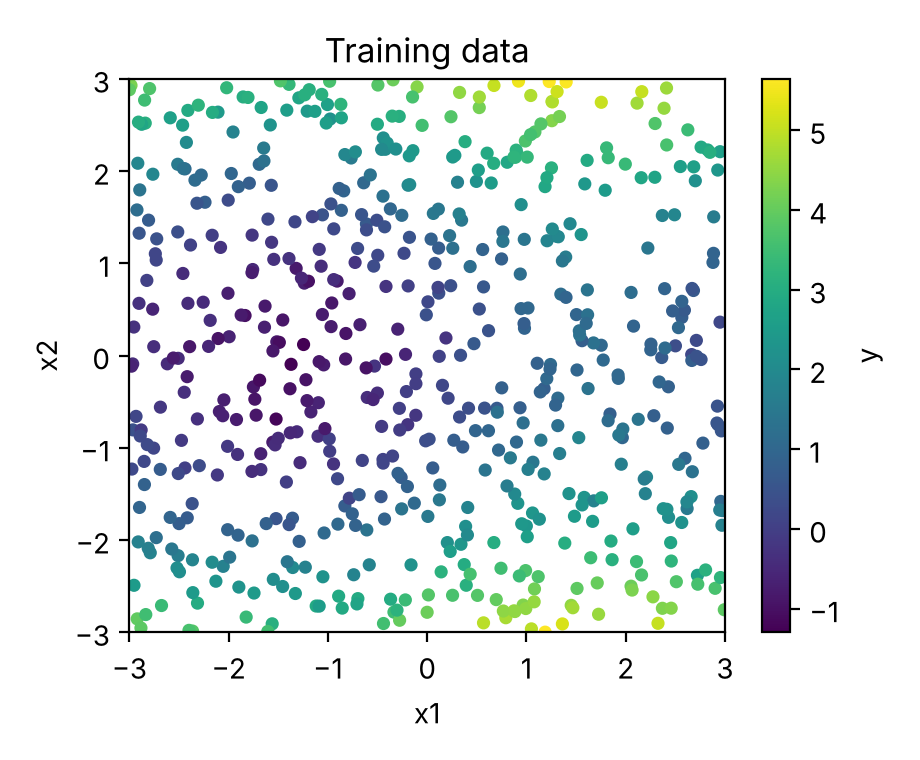
\includegraphics[width=0.45\linewidth]{../figures/q3a_train.png}
\end{center}

\textbf{3(b)}
For $j=1,\dots,h$ draw $w_j\sim N(0,I_2/\sigma^2)$ and $b_j\sim U[0,2\pi]$, and let
\[
\phi(x)=\big(\sin(w_1^\top x+b_1),\cos(w_1^\top x+b_1),\dots,\sin(w_h^\top x+b_h),\cos(w_h^\top x+b_h)\big)^\top,\qquad D=2h.
\]
With design matrix $\Phi$ and a separate intercept, fit
\[
(\hat\beta,\hat a)=\arg\min_{\beta,a}\ \frac1n\|y-\Phi\beta-a\mathbf 1\|_2^2+\lambda\|\beta\|_2^2.
\]
I fix $D=1000$ and $\lambda=10^{-3}$ and sweep $\sigma$. Very small $\sigma$ gives high-frequency features and severe overfitting (training MSE about $10^{-4}$ but validation MSE about 6.9 at $\sigma=0.05$); very large $\sigma$ oversmooths. The best value is $\sigma=3$, with validation MSE 0.0359.

\begin{center}
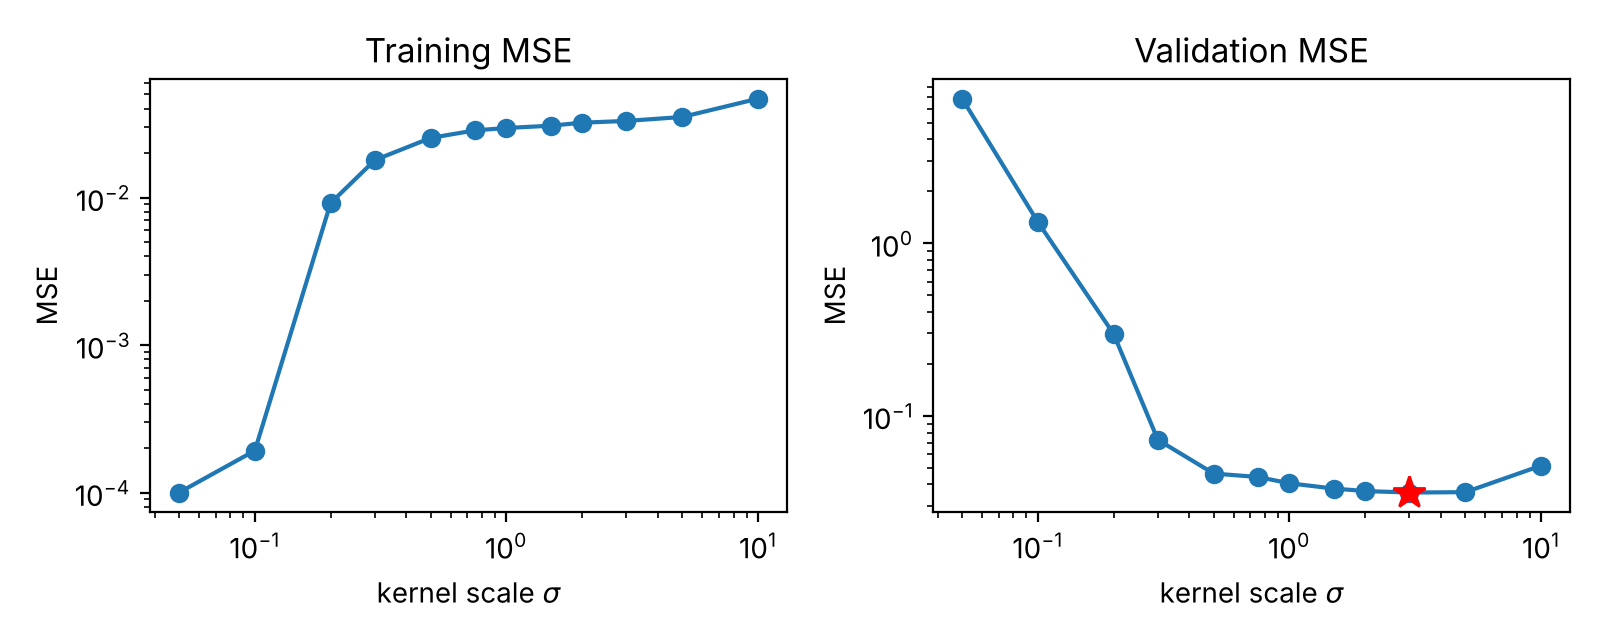
\includegraphics[width=0.85\linewidth]{../figures/q3b_rks_sweep.png}
\end{center}

\textbf{3(c)}
The MLP is $f_\theta(x)=a^\top\mathrm{ReLU}(Wx+b)+c$, trained on MSE with Adam (learning rate $10^{-3}$, batch size 64, 1000 epochs). I sweep the hidden width over $\{1,2,4,\dots,512\}$. Widths of 4 or less underfit; from about 16 on, the validation error is nearly flat. The best width is 64, with validation MSE 0.0372.

\begin{center}
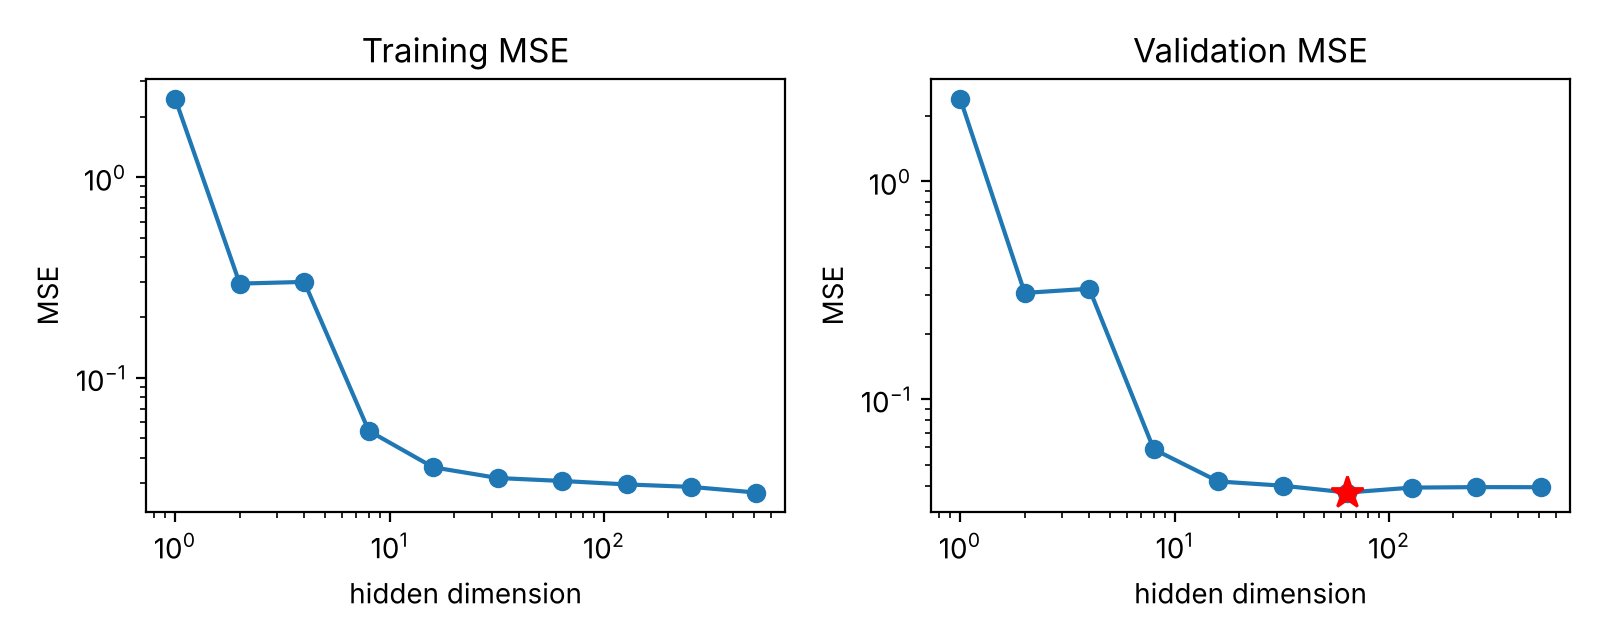
\includegraphics[width=0.85\linewidth]{../figures/q3c_mlp_sweep.png}
\end{center}

\textbf{3(d)}
Refitting both models with the selected hyperparameters on the training set:

\begin{center}
\begin{tabular}{lcc}
\toprule
Model & Training MSE & Validation MSE\\
\midrule
RKS ($D=1000$, $\sigma=3$, $\lambda=10^{-3}$) & 0.0330 & 0.0359\\
MLP (64 hidden units) & 0.0306 & 0.0372\\
\bottomrule
\end{tabular}
\end{center}

RKS has the slightly lower validation MSE (0.0359 vs.\ 0.0372). Both are far better than predicting the training mean (validation MSE 2.40), and a difference of 0.0013 on 200 validation points does not show that one method is generally better. A least-squares fit on $(\sin x_1, x_2^2, 1)$ gives about 0.035, so both models are close to capturing the simple structure of the data. RKS uses fixed smooth random features with a convex ridge fit, while the ReLU MLP learns piecewise-linear features by stochastic optimization.

\begin{center}
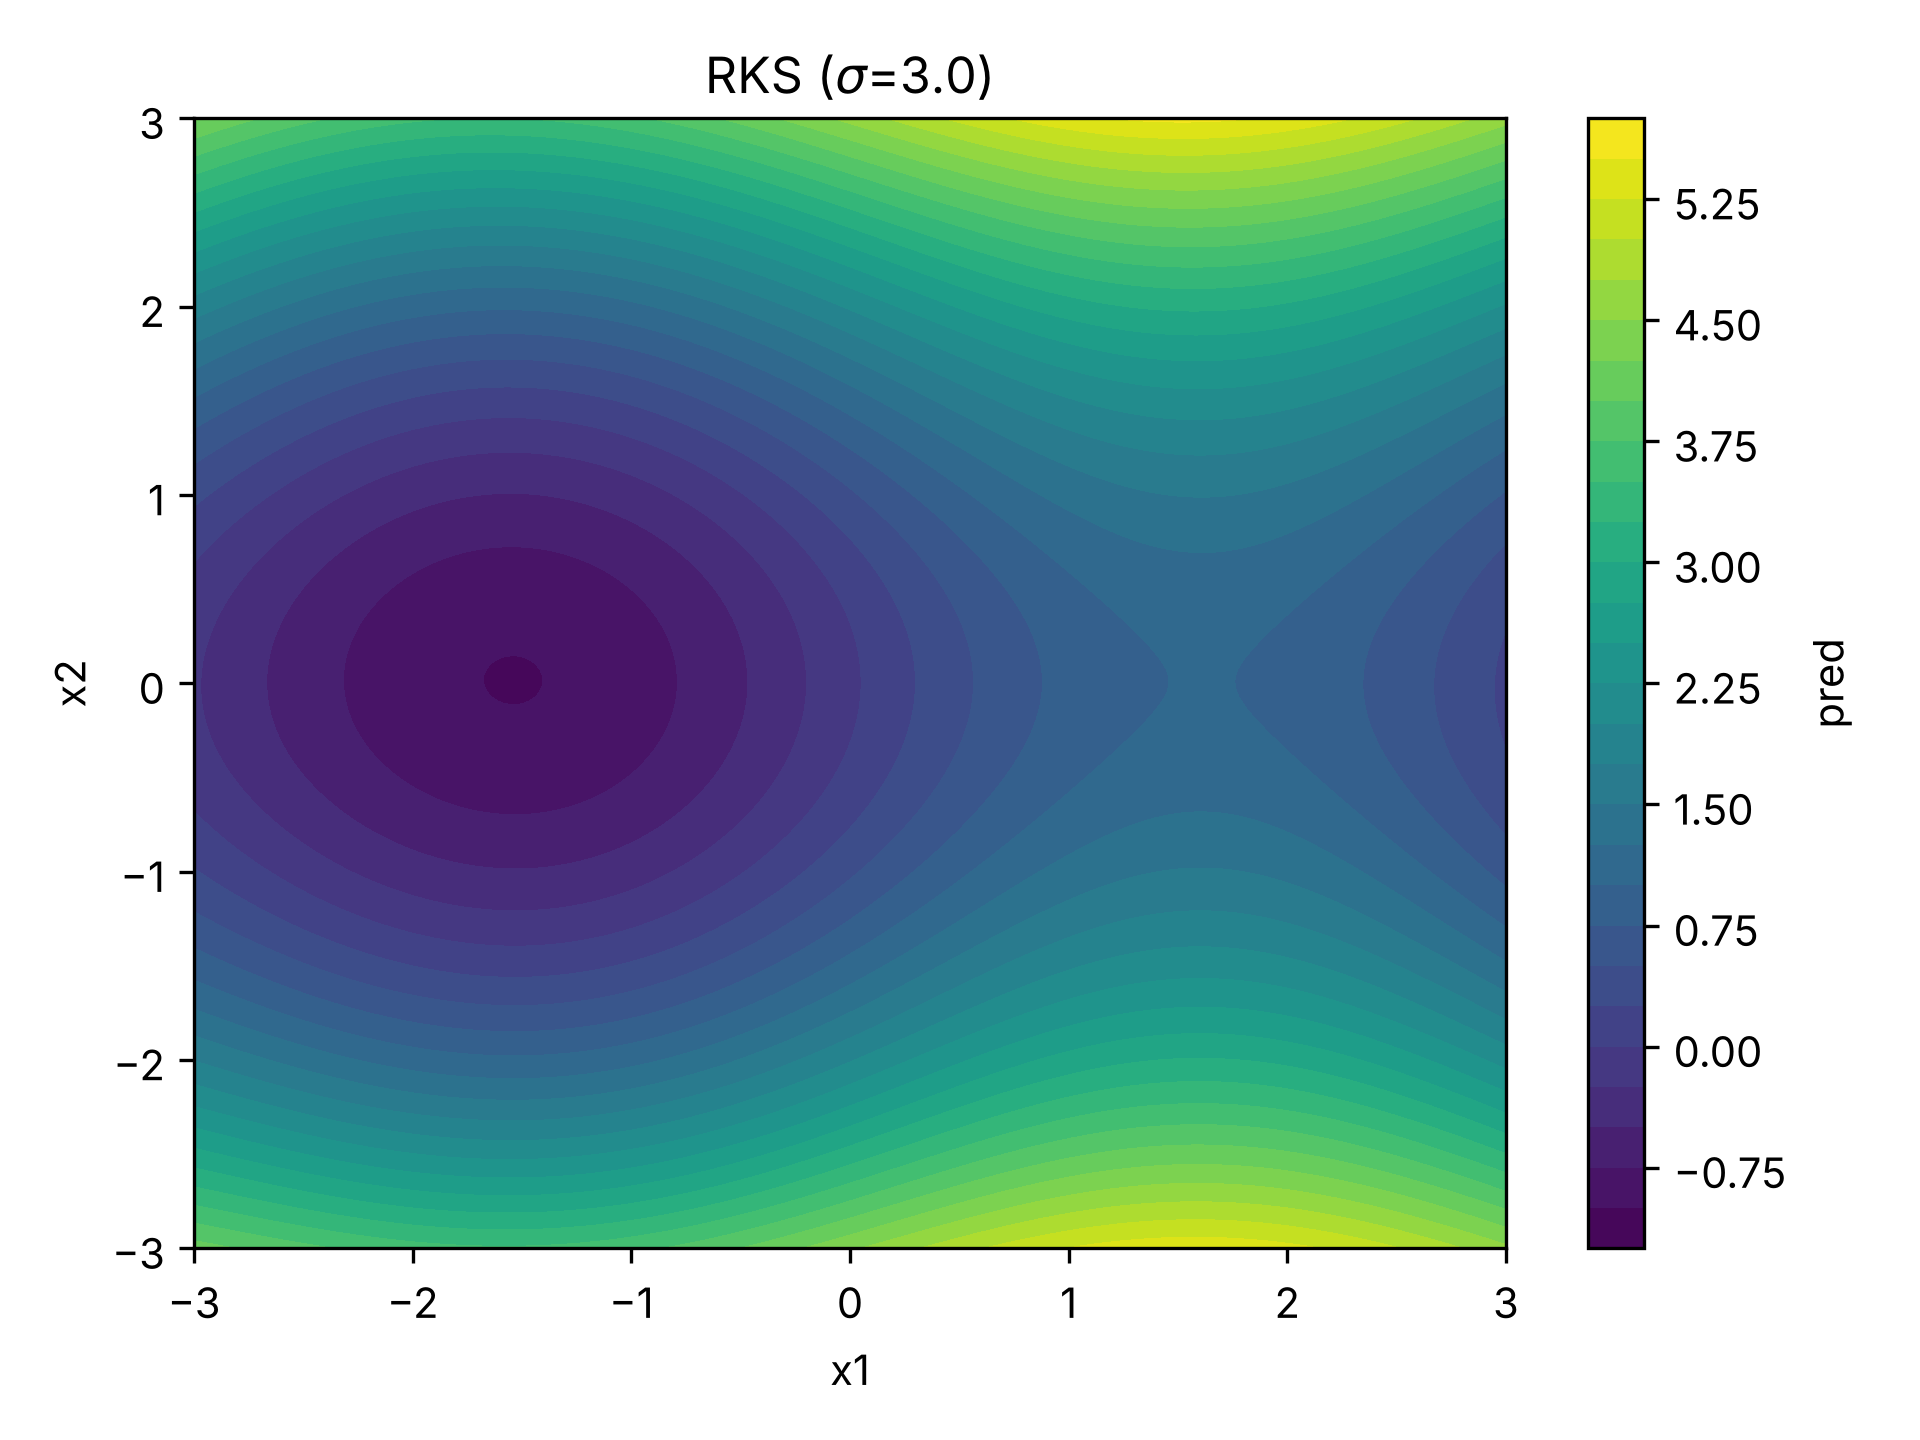
\includegraphics[width=0.45\linewidth]{../figures/q3d_rks_surface.png}\hfill
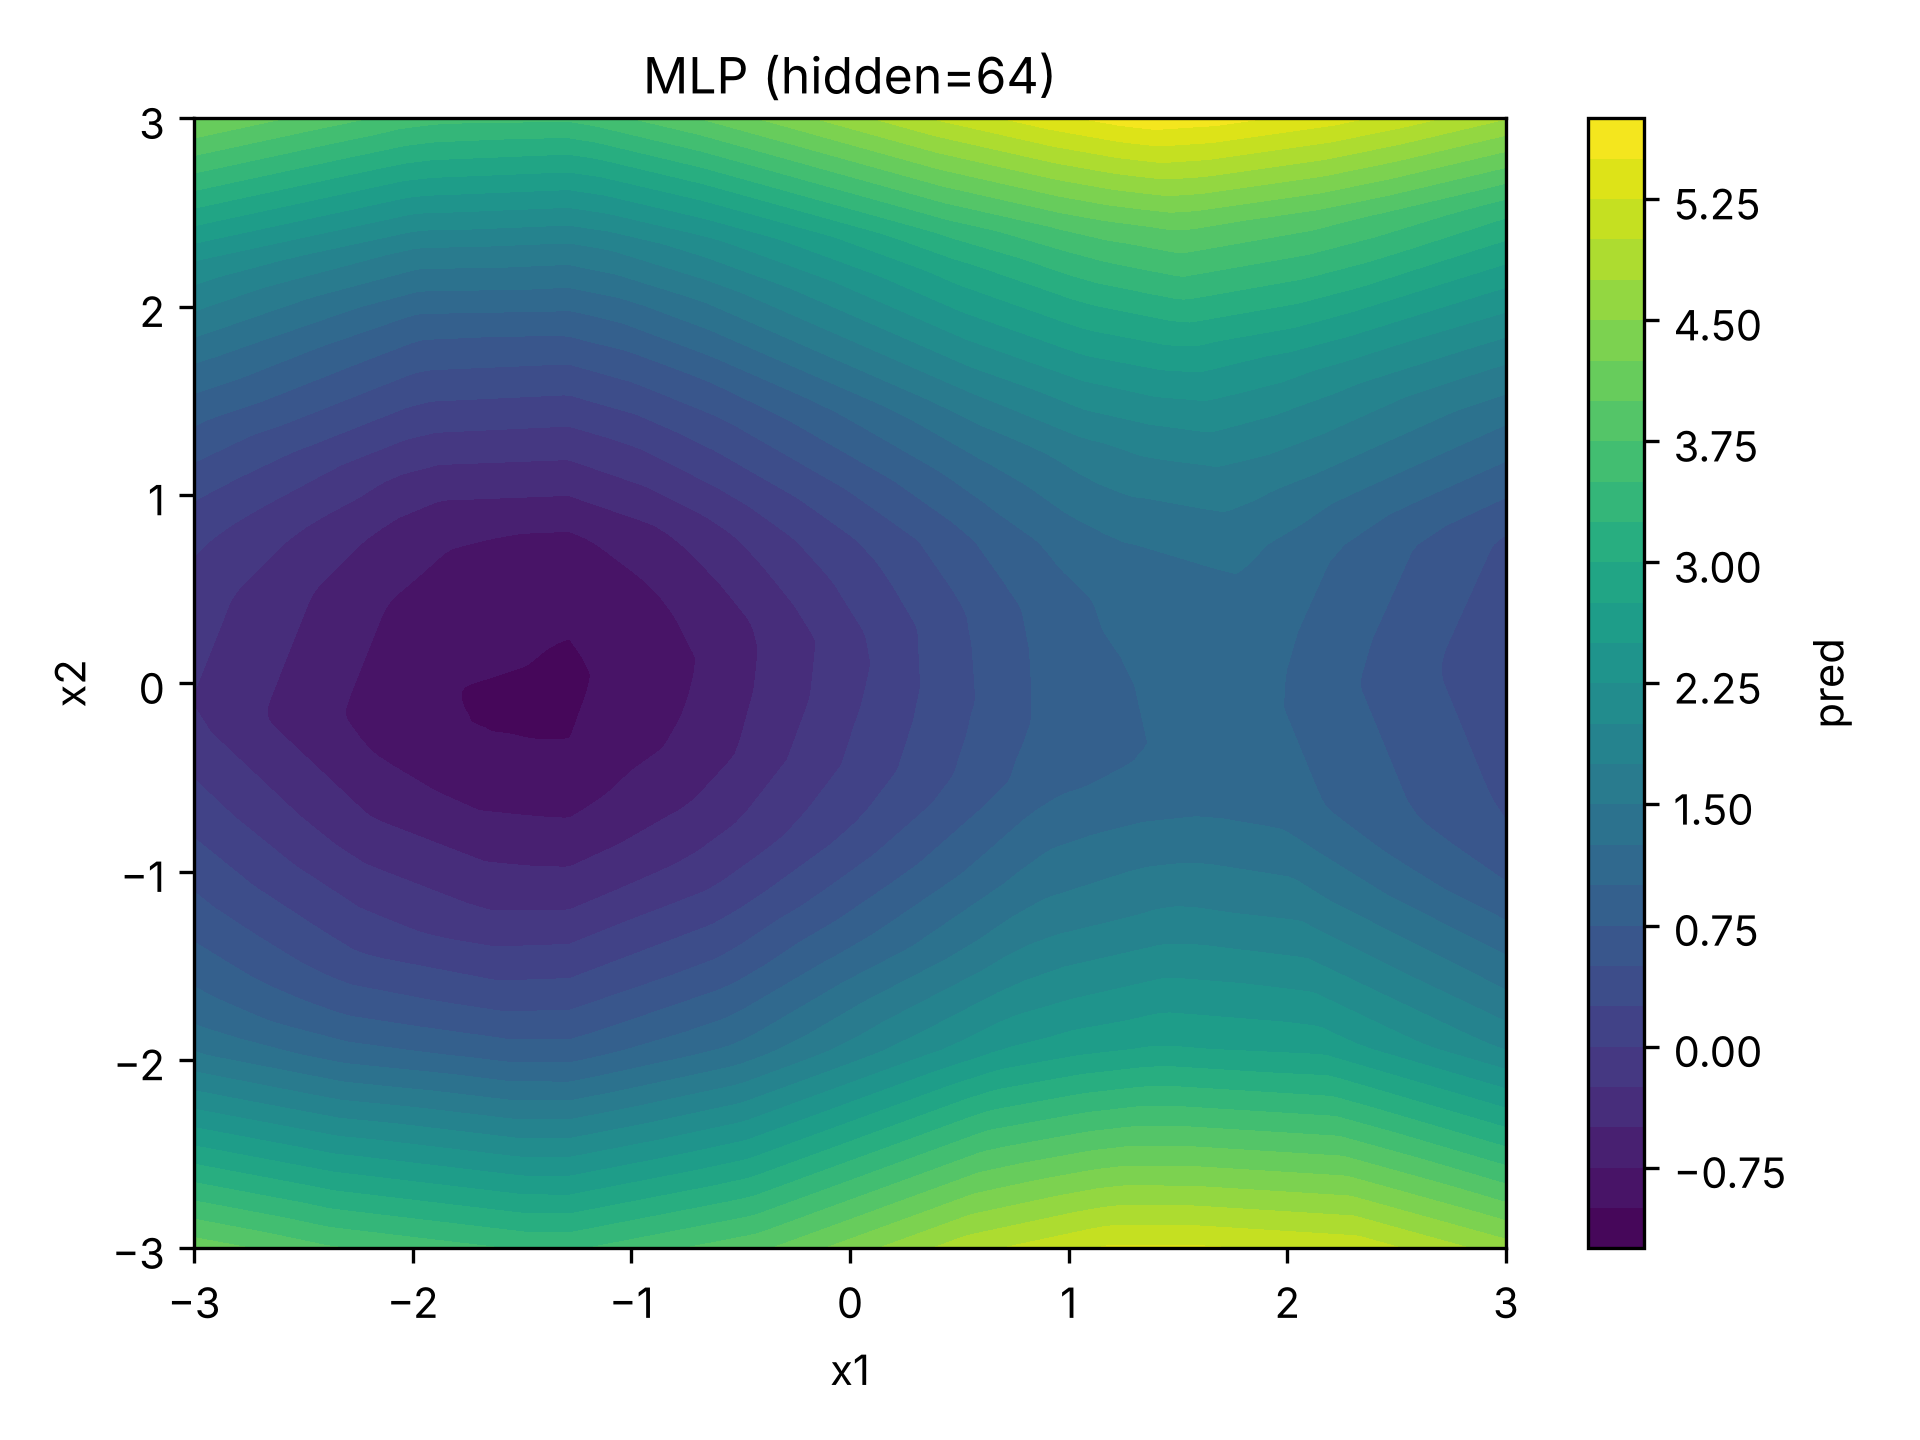
\includegraphics[width=0.45\linewidth]{../figures/q3d_mlp_surface.png}
\end{center}

Both surfaces reproduce the pattern in 3(a): a minimum near $(-1.5,0)$, roughly quadratic growth in $|x_2|$, and high values near $(1.5,\pm3)$. The RKS surface is smooth because it is a sum of sinusoids; the MLP surface is piecewise linear, with polygonal contours. Predictions for the 200 points in test.csv, in the original row order, are submitted as rks\_test\_predictions.csv and mlp\_test\_predictions.csv.

\end{document}
